\documentclass{article}

\usepackage{fancyhdr}
\usepackage{extramarks}
\usepackage{amsmath}
\usepackage{amsthm}
\usepackage{amsfonts}
\usepackage{tikz}
\usepackage[plain]{algorithm}
\usepackage{algpseudocode}

\usetikzlibrary{automata,positioning}

%
% Basic Document Settings
%

\topmargin=-0.45in
\evensidemargin=0in
\oddsidemargin=0in
\textwidth=6.5in
\textheight=9.0in
\headsep=0.25in

\linespread{1.1}

\pagestyle{fancy}
\lhead{\hmwkAuthorName}
\chead{\hmwkClass\ (\hmwkClassInstructor\ \hmwkClassTime): \hmwkTitle}
\rhead{\firstxmark}
\lfoot{\lastxmark}
\cfoot{\thepage}

\renewcommand\headrulewidth{0.4pt}
\renewcommand\footrulewidth{0.4pt}

\setlength\parindent{0pt}

%
% Create Problem Sections
%

\newcommand{\enterProblemHeader}[1]{
    \nobreak\extramarks{}{Problem \arabic{#1} continued on next page\ldots}\nobreak{}
    \nobreak\extramarks{Problem \arabic{#1} (continued)}{Problem \arabic{#1} continued on next page\ldots}\nobreak{}
}

\newcommand{\exitProblemHeader}[1]{
    \nobreak\extramarks{Problem \arabic{#1} (continued)}{Problem \arabic{#1} continued on next page\ldots}\nobreak{}
    \stepcounter{#1}
    \nobreak\extramarks{Problem \arabic{#1}}{}\nobreak{}
}

\setcounter{secnumdepth}{0}
\newcounter{partCounter}
\newcounter{homeworkProblemCounter}
\setcounter{homeworkProblemCounter}{1}
\nobreak\extramarks{Problem \arabic{homeworkProblemCounter}}{}\nobreak{}

%
% Homework Problem Environment
%
% This environment takes an optional argument. When given, it will adjust the
% problem counter. This is useful for when the problems given for your
% assignment aren't sequential. See the last problem of this template for an
% example.
%
\newenvironment{homeworkProblem}[1][-1]{
    \ifnum#1>0
        \setcounter{homeworkProblemCounter}{#1}
    \fi
    \section{Problem \arabic{homeworkProblemCounter}}
    \setcounter{partCounter}{1}
    \enterProblemHeader{homeworkProblemCounter}
}{
    \exitProblemHeader{homeworkProblemCounter}
}

%
% Homework Details
%   - Title
%   - Due date
%   - Class
%   - Section/Time
%   - Instructor
%   - Author
%

\newcommand{\hmwkTitle}{Homework\ \#3}
\newcommand{\hmwkDueDate}{October 2, 2026}
\newcommand{\hmwkClass}{Algorithms}
\newcommand{\hmwkClassTime}{Section B}
\newcommand{\hmwkClassInstructor}{Professor Ada Lovelace}
\newcommand{\hmwkAuthorName}{\textbf{Jane Student}}

%
% Title Page
%

\title{
    \vspace{2in}
    \textmd{\textbf{\hmwkClass:\ \hmwkTitle}}\\
    \normalsize\vspace{0.1in}\small{Due\ on\ \hmwkDueDate\ at 11:59pm}\\
    \vspace{0.1in}\large{\textit{\hmwkClassInstructor\ \hmwkClassTime}}
    \vspace{3in}
}

\author{\hmwkAuthorName}
\date{}

\renewcommand{\part}[1]{\textbf{\large Part \Alph{partCounter}}\stepcounter{partCounter}\\}

%
% Various Helper Commands
%

% Useful for algorithms
\newcommand{\alg}[1]{\textsc{\bfseries \footnotesize #1}}

% For derivatives
\newcommand{\deriv}[1]{\frac{\mathrm{d}}{\mathrm{d}x} (#1)}

% Integral dx
\newcommand{\dx}{\mathrm{d}x}

% Alias for the Solution section header
\newcommand{\solution}{\textbf{\large Solution}}

% Big-O style helpers
\newcommand{\bigO}{\mathcal{O}}

\begin{document}

\maketitle

\pagebreak

\begin{homeworkProblem}
    Show that \(f(n) = 3n^2 + 5n + 2\) is \(\bigO(n^2)\) by giving an explicit
    positive constant \(c\) and threshold \(n_0\) such that \(f(n) \leq c \cdot
    n^2\) for all \(n \geq n_0\).

    \textbf{Solution}

    Take \(n \geq 1\), so \(n \leq n^2\) and \(1 \leq n^2\). Then

    \[
        \begin{split}
            3n^2 + 5n + 2 &\leq 3n^2 + 5n^2 + 2n^2 \\
            &= 10n^2.
        \end{split}
    \]

    So \(c = 10\) and \(n_0 = 1\) satisfy the definition, and \(f(n) \in
    \bigO(n^2)\).
\end{homeworkProblem}

\begin{homeworkProblem}
    Let \(\Sigma = \{a, b\}\). Draw a DFA that accepts every string containing
    the substring \texttt{ab}.

    \textbf{Solution}

    The automaton needs three states: $q_0$ (no progress toward \texttt{ab}),
    $q_1$ (just saw an \texttt{a}), and $q_2$ (accepting; \texttt{ab} has been
    seen).

    \begin{figure}[h]
        \centering
        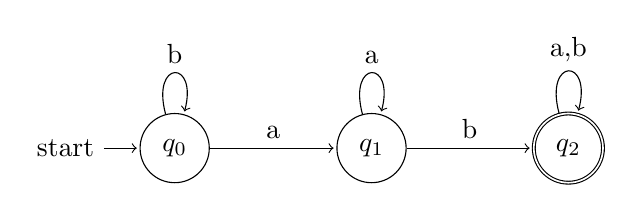
\begin{tikzpicture}[shorten >=1pt,node distance=2.5cm,on grid,auto]
            \node[state, initial] (q0) {$q_0$};
            \node[state] (q1) [right=of q0] {$q_1$};
            \node[state, accepting] (q2) [right=of q1] {$q_2$};
            \path[->]
                (q0) edge [loop above] node {b} (q0)
                     edge node {a} (q1)
                (q1) edge [loop above] node {a} (q1)
                     edge node {b} (q2)
                (q2) edge [loop above] node {a,b} (q2);
        \end{tikzpicture}
        \caption{DFA accepting strings containing \texttt{ab}}
        \label{fig:dfa-ab}
    \end{figure}

    Once the machine reaches $q_2$ it never leaves, so it accepts exactly the
    strings containing \texttt{ab} as a substring.
\end{homeworkProblem}

\begin{homeworkProblem}
    Write pseudocode for \alg{Binary-Search($A, target$)} over a sorted array
    \(A\), returning an index or \(-1\) if \(target\) is absent.

    \textbf{Solution}

    \begin{algorithm}[H]
        \begin{algorithmic}[1]
            \Function{Binary-Search}{$A, target$}
                \State{} $lo \gets 0$, $hi \gets \text{length}(A) - 1$
                \While{$lo \leq hi$}
                    \State{} $mid \gets \lfloor (lo + hi) / 2 \rfloor$
                    \If{$A[mid] = target$}
                        \State{} \Return{} $mid$
                    \ElsIf{$A[mid] < target$}
                        \State{} $lo \gets mid + 1$
                    \Else{}
                        \State{} $hi \gets mid - 1$
                    \EndIf{}
                \EndWhile{}
                \State{} \Return{} $-1$
            \EndFunction{}
        \end{algorithmic}
        \caption{Binary search over a sorted array}
    \end{algorithm}
\end{homeworkProblem}

\pagebreak

\begin{homeworkProblem}
    Prove that \(\sum_{k=1}^{n} k = \dfrac{n(n+1)}{2}\) by induction on \(n\).

    \begin{proof}
        \textbf{Base case} (\(n = 1\)): the left side is \(1\), and the right
        side is \(\frac{1 \cdot 2}{2} = 1\), so the claim holds.

        \textbf{Inductive step}: assume \(\sum_{k=1}^{n} k =
        \frac{n(n+1)}{2}\) for some \(n \geq 1\). Then

        \[
            \sum_{k=1}^{n+1} k = \sum_{k=1}^{n} k + (n+1)
            = \frac{n(n+1)}{2} + (n+1)
            = \frac{(n+1)(n+2)}{2},
        \]

        which is exactly the claimed formula with \(n\) replaced by \(n+1\).
        By induction, the identity holds for every \(n \geq 1\).
    \end{proof}
\end{homeworkProblem}

% Non sequential homework problems: jump to a specific number, then continue.
\begin{homeworkProblem}[7]
    Evaluate \(\int_0^1 (3x^2 - 2x) \, \dx\).

    \textbf{Solution}

    \[
        \int_0^1 (3x^2 - 2x)\,\dx = \left[x^3 - x^2\right]_0^1 = 1 - 1 = 0.
    \]
\end{homeworkProblem}

\end{document}
